\documentclass[10pt,a4paper]{amsart}
\usepackage{amsmath,amssymb,amsthm,graphicx}
\usepackage{amsmath,amsfonts,amssymb,graphicx,xcolor,tikz,bm}
\usetikzlibrary{arrows.meta,shapes.geometric}
\usepackage[backend=biber]{biblatex}
\addbibresource{items/ALCO468-references-r002.bib}
%\theoremstyle{plain}
\theoremstyle{definition}
\newtheorem{theorem}{Theorem}[section]
\newtheorem{proposition}[theorem]{Proposition}
\newtheorem{claim}[theorem]{Claim}
\newtheorem{lemma}[theorem]{Lemma}
\newtheorem{corollary}[theorem]{Corollary}
\newtheorem{problem}[theorem]{Problem}
\newtheorem{conjecture}[theorem]{Conjecture}
\newtheorem{definition}[theorem]{Definition}
\newtheorem{example}[theorem]{Example}
\newtheorem{algorithm}[theorem]{Algorithm} 
\newtheorem{procedure}[theorem]{Procedure}
\newtheorem{observation}[theorem]{Observation}
\newtheorem{case}{Case}
\newtheorem{xca}[theorem]{Exercise}
\newtheorem{consequence}[theorem]{Consequence}
\newtheorem{definition/theorem}[theorem]{Definition/Theorem}

\theoremstyle{remark}
\newtheorem{remark}[theorem]{Remark}
\newtheorem{notation}[theorem]{Notation}


\numberwithin{equation}{section}
\renewcommand{\labelitemi}{$\circ$} % A typesetting pun?!
\setcounter{MaxMatrixCols}{20}


%%%%%%blackboard letters
\newcommand{\bC}{\mathbb{C}}
\newcommand{\bN}{\mathbb{N}}
\newcommand{\bK}{\mathbb{K}}
\newcommand{\bP}{\mathbb{Z}_+} 
\newcommand{\bQ}{\mathbb{Q}}
\newcommand{\bR}{\mathbb{R}}
\newcommand{\bZ}{\mathbb{Z}}
\newcommand{\ka}{\kappa}
\newcommand{\la}{\lambda}
\newcommand{\bx}{\bm x}
\newcommand{\tre}{\textcolor{red}}
\newcommand{\tgr}{\textcolor{green}}
\newcommand{\dom}{\unrhd}
\newcommand{\domby}{\unlhd}

\DeclareMathOperator{\Asc}{Asc}
\DeclareMathOperator{\asc}{asc}
\DeclareMathOperator{\Inv}{Inv}
\DeclareMathOperator{\inv}{inv}
\DeclareMathOperator{\Fix}{Fix}
\DeclareMathOperator{\HT}{HT}
\DeclareMathOperator{\sgn}{sgn}

%:Sym definitions
\newcommand{\Sym}{\ensuremath{\operatorname{Sym}}}

%: compositions and tableaux
\newcommand\ol[1]{\overline{#1}}
\newcommand\ul[1]{\underline{#1}}
\newcommand\ch[1]{\check{#1}}
\newcommand\strongof[1]{{#1}^+}
\newcommand\partitionof[1]{\widetilde{#1}}
\newcommand\reverse[1]{{#1}^*}
\newcommand\ccomplement[1]{{#1}^c}
\newcommand\ctranspose[1]{{#1}^t}

% Others
\newcommand{\ra}{r_\alpha}
\newcommand{\rb}{r_\beta}
\newcommand{\bd}{P_{R,S}}
\newcommand{\lah}{\hat{\lambda}}
\newcommand{\al}{\alpha}


\newcommand*\circled[1]{\tikz[baseline=(char.base)]{
            \node[shape=circle,draw,inner sep=2pt] (char) {#1};}}
%%% tableau macros %%%
\newlength\cellsize \setlength\cellsize{15\unitlength}
\savebox2{%
\begin{picture}(15,15)
\put(0,0){\line(1,0){15}}
\put(0,0){\line(0,1){15}}
\put(15,0){\line(0,1){15}}
\put(0,15){\line(1,0){15}}
\end{picture}}
\newcommand\cellify[1]{\def\thearg{#1}\def\nothing{}%
\ifx\thearg\nothing
\vrule width0pt height\cellsize depth0pt\else
\hbox to 0pt{\usebox2\hss}\fi%
\vbox to 15\unitlength{
\vss
\hbox to 15\unitlength{\hss$#1$\hss}
\vss}}
\newcommand\tableau[1]{\vtop{\let\\=\cr
\setlength\baselineskip{-16000pt}
\setlength\lineskiplimit{16000pt}
\setlength\lineskip{0pt}
\halign{&\cellify{##}\cr#1\crcr}}}
\savebox3{%
\begin{picture}(15,15)
\put(0,0){\line(1,0){15}}
\put(0,0){\line(0,1){15}}
\put(15,0){\line(0,1){15}}
\put(0,15){\line(1,0){15}}
\end{picture}}
\newcommand\expath[1]{%
\hbox to 0pt{\usebox3\hss}%
\vbox to 15\unitlength{
\vss
\hbox to 15\unitlength{\hss$#1$\hss}
\vss}}
\newcommand\bas[1]{\omit \vbox to \cellsize{ \vss \hbox to \cellsize{\hss$#1$\hss} \vss}}

\newcommand{\emt}{\mbox{ }}
\AtBeginDocument{\renewcommand{\shorttitle}{Elementary top coefficients of natural unit interval graphs}}
\title{Product formula for the elementary top coefficient of a natural unit interval graph (Original Theorem3.11)}
\author{Bruce E. Sagan, Foster Tom}
\date{arxiv:2407.06155; CC BY4.0}
\begin{document}
\maketitle
\noindent\textit{Editorial note.} One count only: exactv1 Theorem3.11. All movable-entry lemmas, involution and fixed-point induction are uncounted supporting current author core.\par\medskip
\noindent\textit{Editorial note.} Selected math is exact arXivv1, not the later revised ALCO version. Historical conjecture wording in the v1 introduction is retained as historical source text.\par\medskip
\noindent\textit{Editorial note.} No author proof was supplied by the assistant. The complete selected argument uses the original prior Schur expansion and dual Jacobi–Trudi identity. The omitted routine-compositions discussion in unrelated Theorem3.16 is outside selected assembly and dependencies.\par\medskip
\noindent\textit{Editorial note.} Author source slips such as Lemma3.7(a), Fix phi\_G rather than phi\_G-prime in a sentence, and the original induction exponent are retained without mathematical correction.\par\medskip
\noindent\textit{Editorial note.} Inline author TikZ/picture/tableau graphics are retained. Only presentation counters and a standard-package wrapper were added; the biblatex backend is changed from bibtex to biber. Original source/bibliography remain saved.\par\medskip
\noindent\textit{Editorial note.} r002 technical bibliography repair only: in markedgraphs, replace comma-separated author-list syntax by BibTeX and separators for Aliste-Prieto, J.; de Mier, A.; Orellana, R.; Zamora, J. All four authors, entry key, title, arXiv2202.11787 and year2022 are retained. Original references.bib and preamble.tex remain unchanged; task-r001.json preserves the prior task. No mathematical source or bibliography entry is removed.\par\medskip
\noindent\textit{Editorial note.} Presentation-only layout revision: preserve all author mathematics and full front title; allow paragraph stretch or use a short running title to prevent verified clipping.\par\medskip
\noindent\textit{Editorial scope.} One main coefficient product formula, with complete current involution and weighted fixed-point induction. Faithful collection only, not author mathematical certification.\par\medskip
\noindent\textit{Allowed standard prerequisites (editorial).}\begin{itemize}
\item Shareshian–Wachs Schur expansion for natural unit interval graphs. Original Theorem3.2, cited chromposquasi Theorem6.3, complete statement retained at native687–695. Prior q-weighted G-tableau expansion is accepted as the established input; current hook involution and fixed-point classification are fully retained.
\item Dual Jacobi–Trudi identity and ordinary symmetric-function basis conventions. Native706–723, cited Sagan Theorem4.5.1 and Stanley Corollary7.16.2; original determinant and hook reduction retained. Standard basis identity. No current movable-entry or induction obligation is delegated to it.
\item Earlier acyclic-orientation coefficient identity. Original native401–422 cites Stanley Theorem3.3 and Shareshian–Wachs Theorem5.3. Context for §3 first sentence only; the selected proof proceeds through author tableaux, not the later unrelated orientation bijection.
\end{itemize}\medskip
\section{Introduction}\label{section:introduction}
Let $G=(V,E)$ be a graph with vertex set $V=\{v_1,\ldots,v_n\}$ and edge set $E$.
Also let $\bm x=\{x_1,x_2,\ldots\}$ be a set of commuting variables indexed by the positive integers $\mathbb N$.
In his groundbreaking 1995 work, Stanley defined the \emph{chromatic symmetric function} \cite[Definition 2.1]{chromsym}
$$
X_G(\bm x)=\sum_\kappa x_{\kappa(v_1)}\cdots x_{\kappa(v_n)},
$$
where the sum is over all \emph{proper colourings} of $G$, which are functions $\kappa:V\to\mathbb N$ such that whenever $ij\in E$, we have $\kappa(i)\neq\kappa(j)$. Consider the expansion 
\begin{equation}
\label{c_la}
X_G(\bm x)=\sum_\lambda c_\lambda e_\lambda
\end{equation}
in the basis of \emph{elementary symmetric functions}. 
We reserve the notation $c_\la$ for these coefficients.
We say that $X_G(\bx)$ is \emph{$e$-positive} if all the $c_\la$ are nonnegative, that is, every $e_\la$ which appears does so with positive coefficient.
Stanley and Stembridge  \cite[Conjecture 5.1]{chromsym}, \cite[Conjecture 5.5]{stanstem} made the following conjecture which has become one of the driving forces behind the study of $X_G(\bx)$.
\begin{conjecture}[$(\bm 3+\bm 1)$-free Conjecture]
\label{SSconj}
 If $G$ is the incomparability graph of a $(\bm 3+\bm 1)$-free poset, 
 then $X_G(\bm x)$ is $e$-positive.
\end{conjecture}
Guay-Paquet \cite[Theorem 5.1]{stanstemreduction} showed that it suffices to prove $e$-positivity whenever $G$ is the incomparability graph of a 
poset which is both $(\bm 3+\bm 1)$- and $(\bm 2+\bm 2)$-free.  These are called {\em unit interval graphs}. Shareshian and Wachs defined a $q$-analogue of $X_G(\bm x)$~\cite[Definition 1.2]{chromposquasi} as follows.
Suppose $G$ has vertex set $V=[n]:=\{1,\ldots,n\}$.  Now a proper coloring 
$\ka:[n]\rightarrow\mathbb N$ has {\em ascent number}
$$
\asc\ka = \#\{ ij \in E \mid i<j \text{ and } \ka(i)<\ka(j)\},
$$
where we will use a hash tag or a pair of vertical bars to denote cardinality.  Now define the \emph{chromatic quasisymmetric function} to be
$$
X_G(\bm x;q)=\sum_\kappa q^{\text{asc}(\kappa)}x_{\kappa(1)}\cdots x_{\kappa(n)},
$$
summed over proper $\ka:[n]\rightarrow\mathbb N$.
To generalize Conjecture~\ref{SSconj} to this setting, it suffices to consider unit interval graphs with a particular labeling.  Say that $G=([n],E)$ is a {\em natural unit interval graph}  if for all $1\leq i<j<k\leq n$ we have
\begin{equation}\label{eq:uicondition}
ik\in E \text{ implies } ij\in E \text{ and } jk\in E.
\end{equation}
Although $X_G(\bm x;q)$ is not generally symmetric in the $\bm x$ variables, Shareshian and Wachs \cite[Theorem 4.5]{chromposquasi} showed that $X_G(\bm x;q)$ is symmetric whenever $G$ is a natural unit interval graph. 
So we have an elementary symmetric function expansion
\begin{equation}
\label{c_la(q)}
X_G(\bm x;q)=\sum_\lambda c_\lambda(q)e_\lambda
\end{equation}
where the $c_\la(q)$ are polynomials in $q$.  
Again, the notation $c_\la(q)$ will always refer to these coefficients.
Call the expansion {\em $e$-positive} if the coefficients in each $c_\la(q)$ are nonnegative.
This leads to the following conjecture.
\begin{conjecture}[Shareshian-Wachs]
\label{SWconj}
 If $G$ is a natural unit interval graph
 then $X_G(\bm x;q)$ is $e$-positive.
\end{conjecture}
Note that when we set $q=1$ we recover Conjecture~\ref{SSconj}, so $c_\lambda(1)=c_\lambda$.
Several authors proved $e$-positivity for particular classes of natural unit interval graphs $G$. Harada and Precup \cite[Theorem 6.1]{stanstemhess} proved that $X_G(\bm x;q)$ is $e$-positive whenever $G$ has independence number $2$ using cohomology of abelian Hessenberg varieties and Cho and Huh \cite[Theorem 3.3]{chromstoe} gave a purely combinatorial proof. Cho and Hong \cite[Theorem 1.8]{chrombounce3} proved that $X_G(\bm x)$ is $e$-positive whenever $G$ has independence number $3$. Dahlberg \cite[Corollary 5.4]{trilad} proved that $X_G(\bm x)$ is $e$-positive whenever $G$ has clique number $3$. Gebhard and Sagan \cite[Corollary 7.7]{chromnsym} proved that $X_G(\bm x)$ is $e$-positive whenever $G$ is formed by joining a sequence of cliques at single vertices and Tom \cite[Corollary 4.20]{qforesttriples} proved that $X_G(\bm x;q)$ is $e$-positive for such graphs by finding an explicit formula. 

One can alternatively take a dual approach to the Stanley--Stembridge conjecture by fixing a particular partition $\lambda$ and proving nonnegativity of $c_\lambda(q)$ or $c_\lambda$ for all natural unit interval graphs $G$. Hwang \cite[Theorem 5.13]{chromtwoparthook} proved that $c_\lambda(q)$ is nonnegative whenever $\lambda$ is a hook. Abreu and Nigro \cite[Corollary 1.10]{chromhesssplitting} and independently Rok and Szenes \cite[Theorem 4.1]{chromeschers} proved that $c_\lambda$ is nonnegative whenever $\lambda$ has exactly two rows. Clearman, Hyatt, Shelton and Skandera \cite[Theorem 10.3]{chromhecke} proved that $c_\lambda(q)$ is nonnegative whenever $\lambda$ has exactly two columns, using a connection to characters of Hecke algebras. 



\setcounter{section}{2}
\setcounter{equation}{3}
\setcounter{figure}{0}

\begin{figure}
$$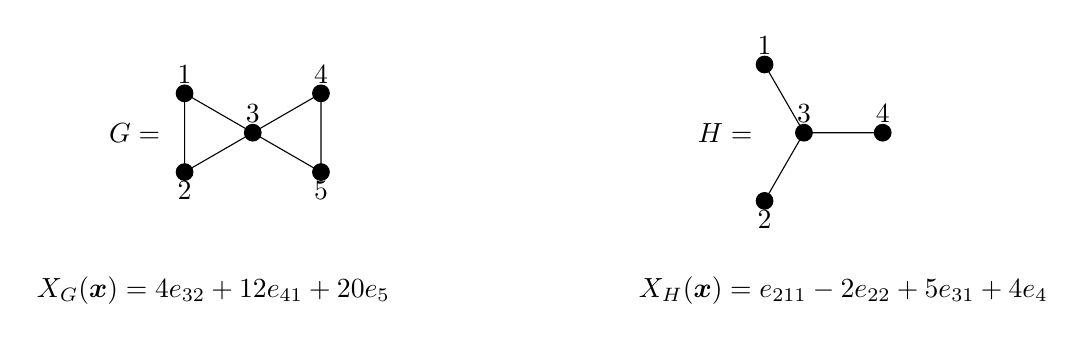
\begin{tikzpicture}
\draw (0,0) node (1){$G=$};
\filldraw (0.634,0.5) circle (3pt) node[align=center,above] (1){1};
\filldraw (0.634,-0.5) circle (3pt) node[align=center,below] (2){2};
\filldraw (1.5,0) circle (3pt) node[align=center,above] (3){3};
\filldraw (2.366,0.5) circle (3pt) node[align=center,above] (4){4};
\filldraw (2.366,-0.5) circle (3pt) node[align=center,below] (5){5};
\draw (0.634,0.5)--(0.634,-0.5)--(1.5,0)--(0.634,0.5) (2.366,0.5)--(2.366,-0.5)--(1.5,0)--(2.366,0.5);
\draw (7.5,0) node (1) {$H=$};
\draw (8,0.866)--(8.5,0) (8,-0.866)--(8.5,0) (8.5,0)--(9.5,0);
\filldraw (8,0.866) circle (3pt) node[align=center,above] (1){1};
\filldraw (8,-0.866) circle (3pt) node[align=center,below] (2){2};
\filldraw (8.5,0) circle (3pt) node[align=center,above] (3){3};
\filldraw (9.5,0) circle (3pt) node[align=center,above] (4){4};
\draw (1,-2) node (){$X_G(\bm x)=4e_{32}+12e_{41}+20e_5$};
\draw (9,-2) node (){$X_H(\bm x)=e_{211}-2e_{22}+5e_{31}+4e_4$};
\end{tikzpicture}
$$
\caption{\label{fig:alphaomegaexample} The bowtie graph, the claw graph, and their chromatic symmetric functions}
\end{figure}

Recall that an \emph{acyclic orientation} of $G=([n],E)$ is an assignment $O$ of directions to each edge of $G$ such that there are no directed cycles. 
Directed edges are also called {\em arcs} and an arc from $i$ to $j$ is denoted $i\to j$.
Vertex $i$ is a \emph{sink} of $O$ if there are no outgoing arcs from $i$.
The {\em ascent set} of $O$ is
$$
\Asc O = \{i\to j \mid i<j\}
$$
with {ascent number}
$$
\asc O =\#\Asc O.
$$

Stanley \cite[Theorem 3.3]{chromsym} proved that for an arbitrary graph $G$, the sum 
\begin{equation}
\label{eq:ao}
a_j:=\sum_{\lambda: \ \lambda'_1=j}c_\lambda
\end{equation}
is the number of acyclic orientations of $G$ with exactly $j$ sinks. Shareshian and Wachs \cite[Theorem 5.3]{chromposquasi} proved that if $G$ is a natural unit interval graph, we have
\begin{equation}
\label{eq:aoq}
a_j(q):=\sum_{\lambda: \ \lambda'_1=j}c_\lambda(q)=\sum_{O: \text{ exactly }j\text{ sinks}}q^{\asc O}.
\end{equation}

Let us say that vertices $u$ and $v$ of a graph $G=([n],E)$ are \emph{equivalent} if they have the same closed neighbourhood. Note that equivalent vertices must be adjacent. We now prove a divisibility result about the coefficients $c_\lambda$ and $c_\lambda(q)$. For an integer $k$ we define the standard $q$-analogues
$$
[k]_q=1+q+q^2+\cdots+q^{k-1}=\frac{q^k-1}{q-1}
$$
and 
$$
[k]_q!=[k]_q[k-1]_q\cdots[2]_q[1]_q.
$$

\setcounter{figure}{3}

\section{The Schur basis}\label{sec:Schur}

If $G$ is a natural unit interval graph then equation~\eqref{eq:aoq} gives an interpretation of the coefficient of $e_n$ in $X_G(\bm x;q)$ as a generating function for the acyclic orientations of $G$ with one sink.
In this section, we use the Schur basis to give another interpretation for the coefficient of $e_n$ in terms of tableaux. 
Throughout this section $G=([n],E)$ will be a natural unit interval graph. Gasharov \cite[Theorem 4]{chrompos31} proved a combinatorial formula for the Schur expansion of $X_G(\bm x)$ in terms of certain tableaux and Shareshian and Wachs \cite[Theorem 6.3]{chromposquasi} proved a $q$-analogue of this result. We will write our Young diagrams in English notation.

\begin{definition}
A \emph{$G$-tableau of shape $\lambda$} is a bijective filling $T$ of the diagram of $\lambda$ with the numbers $1$ through $n$ such that the following two conditions hold.
\begin{enumerate}
\item[(C1)] If an entry $i$ is directly to the left of an entry $j$ in the same row, then $i<j$ and $ij\notin E$.
\item[(C2)] If an entry $i$ is directly above an entry $j$ in the same column, then either $i<j$ or $ij\in E$.
\end{enumerate}
Let $\text{GTab}_\lambda$ denote the set of $G$-tableaux of shape $\lambda$. An \emph{inversion} of $T$ is a pair of entries $(i,j)$ such that
\begin{enumerate}
    \item[(I1)] $i<j$,
    \item[(I2)] $ij\in E$, and
    \item[(I3)] $i$ is in a lower row than $j$.    
\end{enumerate}
We denote by $\Inv T$ the set of inversions of $T$ and $\inv T=\#\Inv T$.
\end{definition}

\begin{theorem}[\cite{chromposquasi}]
\label{thm:Gtab}
The chromatic quasisymmetric function of a natural unit interval graph $G$ satisfies
\begin{equation}
\label{eq:s}
X_G(\bm x;q)=\sum_\lambda\sum_{T\in\text{GTab}_\lambda}q^{\inv T}s_\lambda.
\end{equation}
In particular, $X_G(\bm x;q)$ is Schur-positive.
\end{theorem}

\begin{figure}
\begin{align*}
&\hspace{30pt} \tableau{1&4\\2&5\\3} \hspace{60pt} \tableau{1&5\\2&4\\3} \hspace{90pt} \tableau{2&4\\1&5\\3} \hspace{120pt} \tableau{2&5\\1&4\\3}\\
&\{(3,4),(3,5)\} \hspace{20pt} \{(3,4),(3,5),(4,5)\} \hspace{20pt} \{(1,2),(3,4),(3,5)\} \hspace{20pt} \{(1,2),(3,4),(3,5),(4,5)\}
\end{align*}
\caption{\label{fig:Gtab} The four $G$-tableaux of shape $\lambda=221$ for the bowtie graph $G$}
\end{figure}

\begin{example}

Let $G$ be the bowtie graph from Figure \ref{fig:alphaomegaexample}. The four $G$-tableaux of shape $\lambda=221$ and their inversion sets are given in Figure \ref{fig:Gtab}. By Theorem \ref{thm:Gtab}, the coefficient of $s_{221}$ in $X_G(\bm x;q)$ is $(q^2+2q^3+q^4)$. 
\end{example}

Now we can calculate coefficients in the elementary basis by first using Theorem \ref{thm:Gtab} and then converting Schur functions to elementary symmetric functions using the dual Jacobi--Trudi determinantal identity \cite[Theorem 4.5.1]{symgroup}, \cite[Corollary 7.16.2]{enum2},
\begin{equation}\label{eq:jt}
s_\lambda=\det(e_{\lambda'_i-i+j})_{i,j=1}^{\la_1}.
\end{equation}
In particular, the coefficient of $e_n$ in $s_\lambda$ is nonzero only if $\lambda$ is a \emph{hook}, meaning a partition of the form $\lambda=k1^{n-k}$ for some $1\leq k\leq n$, in which case this coefficient is $(-1)^{k-1}$. Let 
$$
\HT(G)=\{ T \mid \text{$T$ is a $G$-tableau of hook shape}\},
$$
and if $T\in\HT(G)$ has shape $k1^{n-k}$
then define its {\em sign} to be
$$
\sgn T=(-1)^{k-1}. 
$$
By Theorem \ref{thm:Gtab} and \eqref{eq:jt}, the coefficient of $e_n$ in $X_G(\bm x;q)$ is
\begin{equation}\label{eq:cnq}
c_n(q)=\sum_{T\in\HT(G)}(\sgn T) q^{\inv T}.
\end{equation}


We now define a sign-reversing involution $\varphi_G$ on $\HT(G)$ to obtain a positive combinatorial description for $c_n(q)$. The idea will be to move entries between the \emph{arm} and \emph{leg} of $T$, which are the first row and first column of $T$, respectively, excluding the corner entry in the $(1,1)$-cell. We will only move entries if we can preserve the inversion set.

\begin{definition}
Let $T\in\HT(G)$ be a $G$-tableau. An entry $j$ in the arm of $T$ is \emph{movable} if it can be moved to the leg of $T$ to produce a tableau 
$T^j$ such that
\begin{enumerate}
    \item[(M1)] $T^j\in\HT(G)$, and
    \item[(M2)] $\Inv T^j=\Inv T$.
\end{enumerate}
Similarly,  entry $j$ is {\em movable} from the leg to the arm if the resulting tableau $T^j$ satisfies (M1) and (M2).

\end{definition}

We will see shortly that if $j$ is movable then the position to which $j$ can be moved, and hence $T^j$, are uniquely determined.

\begin{example}

In the first line of Figure~\ref{move} we see a natural unit interval graph, $G$, and one of its $G$-tableaux, $T$, of hook shape.  It is easy to check that $\Inv T =\{ (2,3), (4,5)\}$.  Both $3$ and $5$ are movable and the resulting $G$-tableaux are displayed in the second line.  The elements $2$ and $4$ are not 
movable.

\end{example}

\begin{figure}
\begin{center}
\begin{tikzpicture}
\draw(-2,0) node{$G=$};
\filldraw(-1,0) circle(.1);
\draw(-1,-.3) node{$1$};
\filldraw(0,0) circle(.1);
\draw(0,-.3) node{$2$};
\filldraw(1,0) circle(.1);
\draw(1,-.3) node{$3$};
\filldraw(2,0) circle(.1);
\draw(2,-.3) node{$4$};
\filldraw(3,0) circle(.1);
\draw(3,-.3) node{$5$};
\draw plot [smooth, tension=2] coordinates {(0,0) (1,.7) (2,0)};
\draw (-1,0)--(3,0);
\draw(5.5,0) node{$T=$};
\draw (7,0) node{\tableau{1 & 3 & 5\\ 2\\ 4}};
\draw(-.5,-2) node{$T^3=$};
\draw(1,-2) node{\tableau{1&5\\ 3\\ 2 \\ 4}};
\draw(3.5,-2) node{$T^5=$};
\draw(5,-2) node{\tableau{1&3\\ 2\\ 5 \\ 4}};
\end{tikzpicture}
\end{center}
\caption{\label{move} A natural unit interval graph $G$, a $G$-tableau $T$, and two $T^j$}
\end{figure}



\begin{lemma} \label{lem:legtoarm}
Let $T\in\HT(G)$ be a $G$-tableau. 

\begin{enumerate}
\item[(a)] An entry $j$ in the leg of $T$ is movable if and only if every entry $i$ of $T$ in a row above $j$ satisfies $ij\notin E$. 
\item[(b)] If the entry $j$ is movable, there is a unique position to which it can be moved and every entry $i$ above $j$ in the leg of $T$ satisfies $i<j$. 
\end{enumerate}

\end{lemma}

\begin{proof}
(a) If $j$ is movable, then we must have $ij\notin E$ for every entry $i$ in the first row of $T$ by (C1) and because $G$ is a natural unit interval graph. We also must have $ij\notin E$ for every entry $i$ in the leg of $T$ above $j$ because otherwise there would be a change in inversions. 

Conversely, suppose that $ij\notin E$ for every entry $i$ above $j$ and let $T^j$ be the tableau obtained by moving $j$ to the arm so that it is strictly increasing, so (C1) holds. We have $\Inv T^j=\Inv T$ because the only change in relative positions occurred between non-adjacent vertices of $G$. If there are entries $x$ and $y$ respectively directly above and below $j$ in $T$, we cannot have $x>y$ and $xy\notin E$ because then either $j>x>y$ and $yj\notin E$ because $G$ is a natural unit interval graph, violating (C2), or $j<x$  and $xj\notin E$ by assumption, again violating (C2). Therefore, the tableau $T^j$ is indeed a $G$-tableau and the entry $j$ is movable.

(b) First note that uniqueness holds because the first row of $T^j$ must be strictly increasing by (C1).  Next, suppose that $j$ is movable and there is an entry $i>j$ above $j$ in the leg of $T$. We have shown that $ij\notin E$ so $i$ must not be directly above $j$ by (C2). Therefore, there is some other entry $i'$ directly above $j$, and $i'j\not\in E$ because $j$ is movable, so $i'<j$. But now because $i>j>i'$, there must be entries $x$ and $y$ in the leg of $T$ above $j$ with $x$ directly above $y$ and $x>j>y$. But because $j$ is movable we have $jx\notin E$, and $xy\notin E$ because $G$ is a natural unit interval graph, which violates (C2).
\end{proof}

\begin{lemma} \label{lem:armtoleg}
Let $T\in\HT(G)$ be a $G$-tableau. Every entry in the arm of $T$ is movable and can be moved to a unique position.
\end{lemma}

\begin{proof}
Let $j$ be an entry in the arm of $T$ and let $x_1,\ldots,x_\ell$ be the entries of the first column of $T$ from top to bottom. By (C1) and the fact that $G$ is a natural unit interval graph, we have $x_1<j$ and $x_1j\notin E$. Therefore, there is some maximal index $i$ with $1\leq i\leq \ell$ such that we have $x_t<j$ and $x_tj\notin E$ for every $1\leq t\leq i$. We claim that the entry $j$ is movable to the position directly below the entry $x_i$. The first row of the resulting tableau $T^j$ satisfies (C1) because $G$ is a natural unit interval graph. We have $x_i<j$ by definition and we cannot have both $x_{i+1}<j$ and $x_{i+1}j\notin E$ by maximality of $i$, so the first column of $T^j$ satisfies (C2). We have $\Inv T^j=\Inv T$ because the entries in the arm of $T^j$ and the entries $x_1,\ldots,x_i$ that are now above $j$ are not adjacent to $j$ so there is no change in inversions. 

Finally, the entry $j$ could not have moved to a higher position because (C2) would not hold by definition of $i$. Also, the entry $j$ could not have moved to a lower position because then it would be movable in $T^j$, which means by Lemma \ref{lem:legtoarm} that $x_{i+1}<j$ and $x_{i+1}j\notin E$, contradicting maximality of $i$.
\end{proof}

Note that by Lemma \ref{lem:legtoarm} and Lemma \ref{lem:armtoleg}, movable entries can be moved to a unique position so the tableau $T^j$ is well-defined, as promised.

\begin{definition}
Let $T\in\HT(G)$ be a $G$-tableau. We define the $G$-tableau
\begin{equation}
\varphi_G(T)=\begin{cases} T&\text{ if }T\text{ has no movable entry,}\\ T^j&\text{ if }T\text{ has smallest movable entry }j.\end{cases}
\end{equation}
We denote by $\Fix\varphi_G$ the set of \emph{fixed points} of $\varphi_G$, meaning those tableaux $T$ for which $\varphi_G(T)=T$.
\end{definition}

We now show that the map $\varphi_G:\HT(G)\to\HT(G)$ is an inv-preserving, sign-reversing involution.

\begin{lemma}\label{lem:signrev}
We have $\varphi_G(\varphi_G(T))=T$ and $\inv \varphi_G(T)=\inv T$ for every $T\in\HT(G)$. Also
$$
\sgn \varphi_G(T) =
\begin{cases}
1   & \text{if $T\in\Fix\varphi_G$,}\\
-\sgn T & \text{else.}
\end{cases}
$$
\end{lemma}

\begin{proof}
This first statement is clear if $T$ has no movable entry because $\varphi_G(T)=T$, so suppose that $T$ has smallest movable entry $j$, so that $\varphi_G(T)=T^j$. We have $\inv T^j=\inv T$ by definition of $\varphi_G$.
By construction, the entry $j$ of $T^j$ is movable and the unique position to which it can be moved was its original position in $T$. However, we need to check that the entry $j$ of $T^j$ is in fact the smallest movable entry. We will show that if a smaller entry $i<j$ of $T^j$ is movable, then $i$ was movable in $T$, contradicting minimality of $j$. 

By Lemma \ref{lem:armtoleg} (a), every entry in the arm of a hook tableau is movable. So if $i$ were in the arm of $T^j$ then it would have been movable in $T$.   Now  suppose that $i$ is in the leg of $T^j$. By Lemma \ref{lem:legtoarm}, the condition for $i$ to be movable is that it is not adjacent to any entries in a higher row. 
So  $i$  movable in $T^j$ but not $T$ means that it is not adjacent to everything above it in $T^j$ but adjacent to something above in  $T$.  This can only happen if $j$ is in the arm of $T$, moves to the leg of $T^j$ below $i$, and $ij\in E$.  But $j$ being movable in $T^j$ implies $ij\notin E$ which is a contradiction.


Finally, if $T\in\Fix\varphi_G$, then $T$ has no movable entry.
By Lemma \ref{lem:armtoleg}, there are no elements in the arm so that $T$ has shape $1^n$ and $\sgn T =1$. If $T\notin\Fix\varphi_G$, then $\varphi_G$ changes the number of columns in passing from $T$ to $\varphi_G(T)$ by exactly one.  It follows that $\sgn \varphi_G(T) = -\sgn T$ which completes the proof.
\end{proof}

\begin{corollary}
Let $G$ be a natural unit interval graph. Then the coefficient of $e_n$ in $X_G(\bm x;q)$ is given by
\begin{equation}
c_n(q)=\sum_{T\in\Fix\varphi_G}q^{\inv T}.
\end{equation}
\begin{proof}
By Lemma \ref{lem:signrev}, the map $\varphi_G$ is an inversion-preserving bijection between the positively-signed non-fixed points and the negatively-signed non-fixed points, so the sum in \eqref{eq:cnq} is equal to the sum over the fixed points, which are positively signed.
\end{proof}
\end{corollary}

We now describe the fixed points of $\varphi_G$ to get an explicit formula for $c_n(q)$ which will follow from Corollary~\ref{qcor} below.


\begin{theorem}\label{thm:coefen}
Let $G=([n],E)$ be a natural unit interval graph. For $2\leq k\leq n$, let $b_k$ denote the number of smaller neighbours of vertex $k$ in $G$. Then the coefficient of $e_n$ in the chromatic quasisymmetric function $X_G(\bm x;q)$ is 
\begin{equation}
c_n(q)=[n]_q[b_2]_q[b_3]_q\cdots[b_n]_q.
\end{equation}
\end{theorem}

By considering the reverse graph obtained by relabeling vertex $k$ to $n-k+1$, we could equivalently think about the number of larger neighbours of each vertex. 

\begin{example}
For the bowtie graph $G$ from Figure \ref{fig:alphaomegaexample}, the coefficient of $e_5$ in $X_G(\bm x;q)$ is \begin{equation}
c_5(q)=[5]_q[2]_q[2]_q=(1+q+q^2+q^3+q^4)(1+q)^2.
\end{equation}
\end{example}

We will use induction on $n$ to enumerate the fixed points of $\varphi_G$. Suppose that $n\geq 2$ and let $G'$ denote the graph $G$ with the vertex $n$ removed. For a tableau $T$ of column shape, we denote by $T_i$ the $i$-th entry from the top.

\begin{lemma}\label{lem:fixind}
If $b_n=0$, then $\Fix\varphi_G=\emptyset$. Otherwise, the tableaux $T\in\Fix\varphi_G$ arise precisely by taking a tableau $T'\in\Fix\varphi_{G'}$ and inserting the entry $n$ either at the bottom, directly above a neighbour of $n$ other than the one occurring highest in $T'$, or at the top if $T'_1$ is a neighbour of $n$. 
\end{lemma}

\begin{proof}
If $b_n=0$, then a $G$-tableau $T\in\text{GTab}_{1^n}$ must have the entry $n$ at the bottom to satisfy (C2).
But then the $n$ is movable by Lemma \ref{lem:legtoarm}. So assume that $b_n\geq 1$. A tableau $T$ constructed from $T'$ in one of the three given ways will satisfy (C2) because $n$ is either at the bottom or directly above a neighbour, and will have no movable elements by Lemma \ref{lem:legtoarm} because $n$ is either at the top or below a neighbour, so we have $T\in\Fix\varphi_G$. We now show that a tableau $T\in\Fix\varphi_G$ must arise in this way. 

Let $T'$ denote the tableau obtained from $T$ by removing the entry $n$. 
We must first show that $T'$ still satisfies (C2).  Suppose, to the contrary, that 
there are entries $x$ and $y$ respectively above and below the entry $n$ in $T$ with $x>y$ and $xy\notin E$. But since  $G$ is a natural unit interval graph this would force $yn\notin E$ since $n>y$.  So $T$ would not satisfy (C2), a contradiction.

Also we claim that  $T'$ has no movable elements. Suppose that $T'$ has a movable element  $j$. By Lemma \ref{lem:legtoarm}, every element $i$ above $j$ in $T'$ must satisfy $i<j$ and $ij\notin E$. Because $j$ is not movable in $T$, the entry $n$ must be above $j$ in $T$ and $jn\in E$ by Lemma \ref{lem:legtoarm} (a). Now every entry $i$ above $n$ in $T$ satisfies $i<j<n$ which implies $in\notin E$ because $G$ is a natural unit interval graph. 
So, by Lemma \ref{lem:legtoarm} (a) again, the only way for $n$ to not be movable in $T$ is if 
$T_1=n$. If $T_2=j$, then $T'_1=j$ so $j$ is not movable in $T'$.  Otherwise, $T_2$ must be some other entry $k$. However, because $k$ is above $j$ in $T'$, we have shown that $k<j$ and $kj\notin E$. 
This  forces $k<n$ and $kn\notin E$ so that $T$ does not satisfy (C2). 
 This final contradiction shows that no element of $T'$ is movable.


Therefore $T'\in\Fix\varphi_G$ and indeed $T$ arises by inserting the entry $n$ somewhere in $T'$. In order to satisfy (C2), the entry $n$ must be inserted either at the bottom or directly above a neighbour of $n$, and in order for $n$ to not be movable, by Lemma \ref{lem:legtoarm}, it must be either at the top or have a neighbour above it.
\end{proof}

Theorem \ref{thm:coefen} follows from the next corollary by summing over $1\leq j\leq n$.

\begin{corollary}
\label{qcor}
Let $G=([n],E)$ be a natural unit interval graph. Then for every $1\leq j\leq n$, we have
\begin{equation}
\sum_{T\in\Fix\varphi_G, \ T_1=j}q^{\inv T}=q^{j-1}[b_2]_q\cdots[b_n]_q.
\end{equation}
\end{corollary}

\begin{proof}
We use induction on $n$, the case of $n=1$ trivial, so suppose that $n\geq 2$. If $b_n=0$, then the statement holds by Lemma \ref{lem:fixind}, so assume that $b_n\geq 1$ and note that because $G$ is a natural unit interval graph, the neighbours of $n$ are exactly $n-b_n,\ldots,n-1$. If $j<n$, then by Lemma \ref{lem:fixind}, every tableau $T\in\Fix\varphi_G$ with $T_1=j$ arises from a tableau $T'\in\Fix\varphi_{G'}$ by inserting the entry $n$ in one of $b_n$ possible positions. Inserting $n$ in the $i$-th place from the bottom results in $(i-1)$ new inversions, so by our induction hypothesis, we have
$$\sum_{T\in\Fix\varphi_G, \ T_1=j}q^{\inv T}=(1+q+\cdots+q^{b_n-1})\sum_{T'\in\Fix\varphi_{G'}, \ T'_1=j}q^{\inv T}=q^{j-1}[b_2]_q\cdots[b_n]_q.$$
If $j=n$, then by Lemma \ref{lem:fixind}, every tableau $T\in\Fix\varphi_G$ with $T_1=n$ arises from a tableau $T'\in\Fix\varphi_G$ with $n-b_n\leq T'_1\leq n-1$ by inserting the entry $n$ at the top. Doing so produces $b_n$ new inversions, so by our induction hypothesis, we have
\begin{align*}\sum_{T\in\Fix\varphi_G, \ T_1=n}q^{\inv T}&=\sum_{i=n-b_n}^{n-1}\sum_{T'\in\Fix\varphi_{G'}, \ T'_1=i}q^{\inv T+b_n}\\&=q^{b_n}\sum_{i=n-b_n}^{n-1}q^{i-1}[b_2]_q\cdots[b_{n-1}]_q=q^{n-1}[b_2]_q\cdots[b_n]_q,\end{align*}
which completes the proof.
\end{proof}

\section{Acknowledgments}
The authors would like to thank Zachary Hamaker, Richard Stanley, and Vincent Vatter for helpful discussions.

\nocite{*}

\printbibliography
\end{document}
